\documentclass{article}
\usepackage{graphicx}
\graphicspath{ {images/} }
\parindent 0pt
\parskip 2ex
\usepackage[margin=0.5in,bottom=1in,top=1in]{geometry}
\usepackage{amsmath}
\usepackage{amssymb}
\usepackage[section]{placeins}
\usepackage{cleveref}
\usepackage{float}

\begin{document}
	
	\begin{titlepage}
	\begin{center}
		\vspace*{1cm}
		
		\Huge
		\textbf{PV Measurement}
		
		\vspace{0.5cm}
		\LARGE
		48550 Renewable Energy Systems - Lab 1
		
		\vspace{1.5cm}
		
		\textbf{Robert Carey}\space\space\space99139382\\
		\textbf{William Rooke}\space\space\space 12051342\\
		\textbf{Joel Goodwin}\space\space\space 98055953\\
		
		\today
		
		\vfill
		
		
		\vspace{0.8cm}
		
		\includegraphics[width=1\textwidth]{uts}
		
		
		
	\end{center}
\end{titlepage}
	\tableofcontents
	\newpage
	\listoffigures
	\listoftables
	\newpage
	
	\section{Purpose}
		\begin{itemize}
			\item To become familiar with the non-linear electrical properties of solar PV generation.
			\item To investigate the effects of solar radiation and shading levels, along with the tilt angle of a solar panel on the electrical characteristics of solar cells.
			\item To determine the optimal conditions for operating a PV panel in a circuit with a known load and understand the maximum power point tracking (MPPT) principle.
			\item To collect measurement data for construction of a PV array for the individual assignment.
		\end{itemize}
	
	\section{Lab Questions}
	\subsection{Q1}
		\textit{Briefly explain the mechanism of solar PV generation with the aid of diagram(s).}
		
		Solar photovoltaic (PV) electricity generation works by using multiple semiconductor devices (PV cells) that convert light into electrical energy. Usually these PV cells are arranged in arrays to increase electrical output.
		
		An example is of PV cell construction is a wafer of p-type silicon with a thin layer of n-type silicon on one side. The p-type and n-type material acts as the positive and negative terminal of the cell respectively. When light hits the PV cell, photons of light provide energy to the electrons to promote them from the valence band into the conduction band, leaving behind a positive electron "hole". At this point, the electrons are now free to flow through the crystal structure and conduct electricity. This process is illustrated in \cref{fig:PVCellStructure}.
		
		\begin{figure}[H]
			\centering
			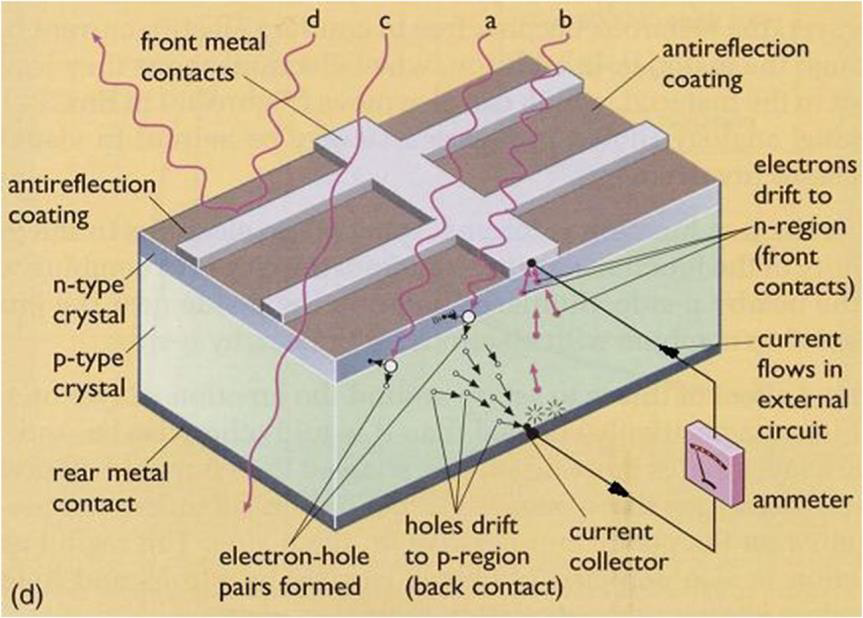
\includegraphics[width=0.5\textwidth]{PVCellStructure}
			\caption{PV Cell Structure}
			\label{fig:PVCellStructure}
		\end{figure}
	
	\newpage
	\subsection{Q2}
		\textit{Explain the three test conditions and show the results in both table format and graphical plots.}
		
		
		We took measurements on two separate days, one with overcast conditions and one with full sun. For both days, we took measurements at the same time of day and location with the solar panel in the same orientation. The tilt angle of the PV panel was changed to provide multiple sets of data.
		
		\begin{enumerate}
			\item Overcast Day
			\begin{itemize}
				\item Solar panel with 0 degrees of tilt.
				\item Solar panel with 40 degrees of tilt.
				\item Solar panel with 90 degrees of tilt.
				\item Solar Panel with 0 degrees of tilt with 3 PV cells covered.
			\end{itemize}
			\item Clear Sunny Day
			\begin{itemize}
				\item Solar panel with 0 degrees of tilt.
				\item Solar panel with 40 degrees of tilt.
			\end{itemize}
		\end{enumerate}	
	
	The results from these test cases can be seen in \cref{section:Results}.
	
	\subsection{Q3}
		\textit{Locate on the graphs the estimated maximum power points (MPPs). Comment on any variation of the MPPs and the implication of loading impedance values for the PV panel to maintain at MPPs under all solar intensity conditions.}
		
		From \cref{fig:VoltagevsPower} it can be seen that the MPP is much larger for higher insolation values (measured in lux). This is due to the fact that there is a much larger current flow occurring with greater insolation.
		
		\Cref{fig:ResistancevsPower} illustrates the implications of loading impedance on the MPP for different insolation. For our higher insolation measurements ($>$38400 Lux), the MPP occurs at impedances of around 50$ \Omega $. However, for lower insolation measurements ($<$8380 Lux), the MPP occurs at impedances of around 250$ \Omega $. This illustrates that in order to maintain the MPP, the load impedance needs to be reduced for greater insolation.
	
	\section{Experimental Measurements}
		To begin taking measurements of the current and voltage produced by the PV panel, the equipment, consisting of the PV panel, a current meter, voltage meter and resistance box, were set up as shown in \cref{fig:circuit}
		\begin{figure}[H]
			\centering
			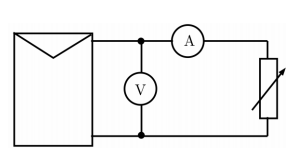
\includegraphics[width=0.5\textwidth]{circuitdiagram}
			\caption{Circuit diagram of experiment}
			\label{fig:circuit}
		\end{figure}
		The insolation of the PV panel was taken for each angle setup by placing the light meter on top of the PV panel before measurements were taken as shown in \cref{fig:lux_reading}.
		\begin{figure}[H]
			\centering
			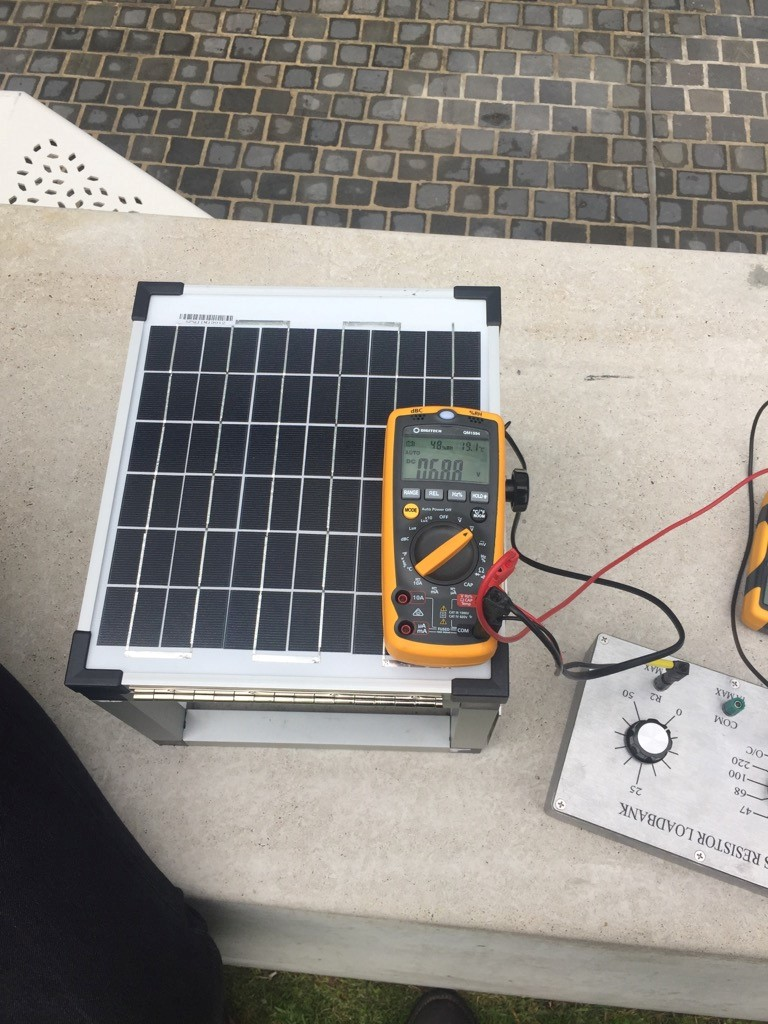
\includegraphics[width=0.3\textwidth]{lux_reading}
			\caption{Measurement of panel insolation}
			\label{fig:lux_reading}
		\end{figure}
		The voltage and current produced by the PV panel was then measured at three different levels of insolation and at a number of resistances, provided by the resistance box, in order to find the maximum power point (MPP) for the panel.
		
	\subsection{Results}\label{section:Results}
	
	\subsubsection{Graphs}
		\begin{figure}[H]
			\centering
			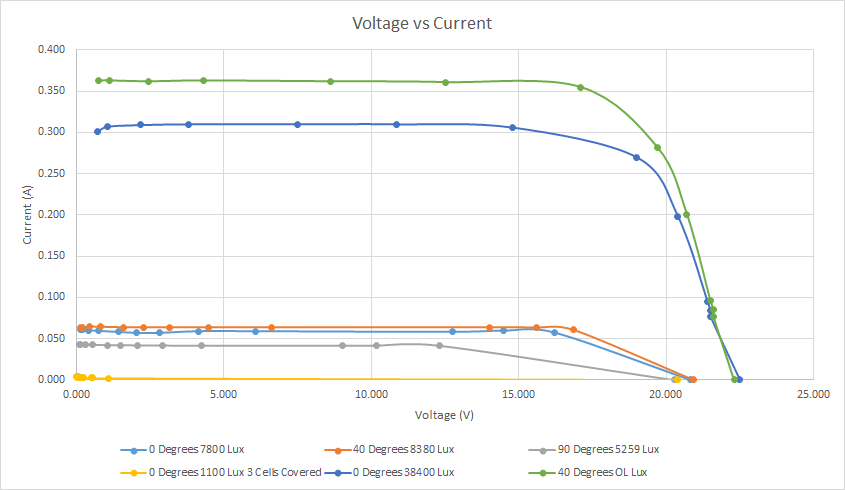
\includegraphics[width=0.8\textwidth]{VoltagevsCurrent}
			\caption{Voltage vs Current}
			\label{fig:VoltagevsCurrent}
		\end{figure}
	
		\begin{figure}[H]
			\centering
			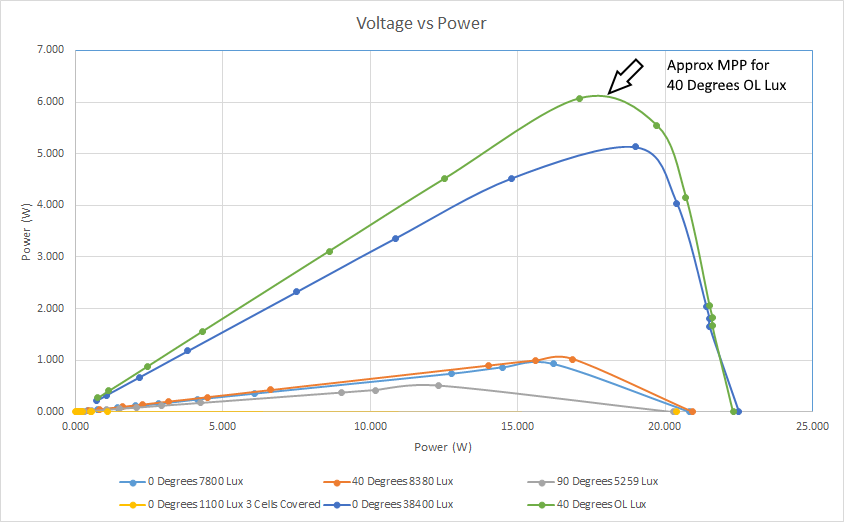
\includegraphics[width=0.8\textwidth]{VoltagevsPower}
			\caption{Voltage vs Power}
			\label{fig:VoltagevsPower}
		\end{figure}
	
		\begin{figure}[H]
			\centering
			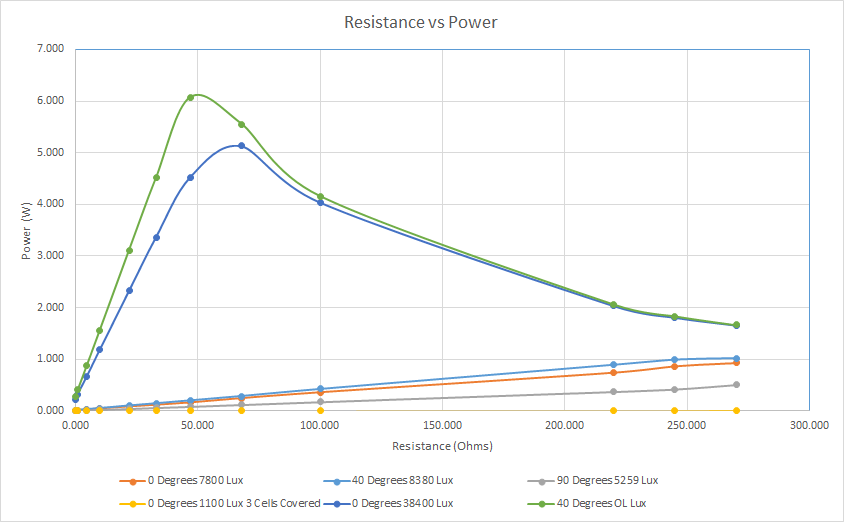
\includegraphics[width=0.8\textwidth]{ResistancevsPower}
			\caption{Resistance vs Power}
			\label{fig:ResistancevsPower}
		\end{figure}
	
	\subsubsection{Tables}
		\begin{table}[H]
			\centering
			\caption{0 Degrees, 7800 Lux}
			\begin{tabular}{|l|l|l|l|l|l|}
				\hline
				
				\textbf{R1 (Ohms)} & \textbf{R2 (Ohms)} & \textbf{Total (Ohms)} & \textbf{Current (A)} & \textbf{Voltage (V)} & \textbf{Power (W)} \\ \hline
				0.00 & 0.00 & 0.00 & 0.06 & 0.14 & 0.01 \\ \hline
				1.00 & 0.00 & 1.00 & 0.06 & 0.20 & 0.01 \\ \hline
				4.70 & 0.00 & 4.70 & 0.06 & 0.43 & 0.03 \\ \hline
				10.00 & 0.00 & 10.00 & 0.06 & 0.74 & 0.04 \\ \hline
				22.00 & 0.00 & 22.00 & 0.06 & 1.43 & 0.08 \\ \hline
				33.00 & 0.00 & 33.00 & 0.06 & 2.03 & 0.12 \\ \hline
				47.00 & 0.00 & 47.00 & 0.06 & 2.83 & 0.16 \\ \hline
				68.00 & 0.00 & 68.00 & 0.06 & 4.15 & 0.24 \\ \hline
				100.00 & 0.00 & 100.00 & 0.06 & 6.08 & 0.36 \\ \hline
				220.00 & 0.00 & 220.00 & 0.06 & 12.75 & 0.74 \\ \hline
				220.00 & 25.00 & 245.00 & 0.06 & 14.50 & 0.87 \\ \hline
				220.00 & 50.00 & 270.00 & 0.06 & 16.20 & 0.93 \\ \hline
				O/C & & & 0.00 & 20.83 & 0.00 \\ \hline
				
			\end{tabular}
		\end{table}
	
		\begin{table}[H]
			\centering
			\caption{40 Degrees, 8380 Lux}
			\begin{tabular}{|l|l|l|l|l|l|}
				\hline
				
				\textbf{R1 (Ohms)} & \textbf{R2 (Ohms)} & \textbf{Total (Ohms)} & \textbf{Current (A)} & \textbf{Voltage (V)} & \textbf{Power (W)} \\ \hline
				0.000 & 0.000 & 0.000 & 0.064 & 0.150 & 0.010 \\ \hline
				1.000 & 0.000 & 1.000 & 0.064 & 0.217 & 0.014 \\ \hline
				4.700 & 0.000 & 4.700 & 0.065 & 0.456 & 0.030 \\ \hline
				10.000 & 0.000 & 10.000 & 0.065 & 0.808 & 0.052 \\ \hline
				22.000 & 0.000 & 22.000 & 0.064 & 1.585 & 0.101 \\ \hline
				33.000 & 0.000 & 33.000 & 0.064 & 2.265 & 0.145 \\ \hline
				47.000 & 0.000 & 47.000 & 0.064 & 3.150 & 0.202 \\ \hline
				68.000 & 0.000 & 68.000 & 0.064 & 4.470 & 0.286 \\ \hline
				100.000 & 0.000 & 100.000 & 0.064 & 6.600 & 0.422 \\ \hline
				220.000 & 0.000 & 220.000 & 0.064 & 14.000 & 0.893 \\ \hline
				220.000 & 25.000 & 245.000 & 0.064 & 15.600 & 0.992 \\ \hline
				220.000 & 50.000 & 270.000 & 0.061 & 16.850 & 1.021 \\ \hline
				O/C & & & 0.000 & 20.930 & 0.000 \\ \hline
				
			\end{tabular}
		\end{table}
	
		\begin{table}[H]
			\centering
			\caption{90 Degrees, 5259 Lux}
			\begin{tabular}{|l|l|l|l|l|l|}
				\hline
				
				\textbf{R1 (Ohms)} & \textbf{R2 (Ohms)} & \textbf{Total (Ohms)} & \textbf{Current (A)} & \textbf{Voltage (V)} & \textbf{Power (W)} \\ \hline
				0.000 & 0.000 & 0.000 & 0.042 & 0.100 & 0.004 \\ \hline
				1.000 & 0.000 & 1.000 & 0.043 & 0.150 & 0.006 \\ \hline
				4.700 & 0.000 & 4.700 & 0.042 & 0.300 & 0.013 \\ \hline
				10.000 & 0.000 & 10.000 & 0.042 & 0.540 & 0.023 \\ \hline
				22.000 & 0.000 & 22.000 & 0.042 & 1.050 & 0.044 \\ \hline
				33.000 & 0.000 & 33.000 & 0.042 & 1.497 & 0.063 \\ \hline
				47.000 & 0.000 & 47.000 & 0.042 & 2.070 & 0.087 \\ \hline
				68.000 & 0.000 & 68.000 & 0.042 & 2.930 & 0.122 \\ \hline
				100.000 & 0.000 & 100.000 & 0.041 & 4.250 & 0.176 \\ \hline
				220.000 & 0.000 & 220.000 & 0.041 & 9.040 & 0.374 \\ \hline
				220.000 & 25.000 & 245.000 & 0.042 & 10.170 & 0.422 \\ \hline
				220.000 & 50.000 & 270.000 & 0.041 & 12.300 & 0.509 \\ \hline
				O/C & & & 0.000 & 20.280 & 0.000 \\ \hline
				
			\end{tabular}
		\end{table}
		
		\begin{table}[H]
			\centering
			\caption{0 Degrees, 1100 Lux, 3 Cells Covered}
			\begin{tabular}{|l|l|l|l|l|l|}
				\hline
				
				\textbf{R1 (Ohms)} & \textbf{R2 (Ohms)} & \textbf{Total (Ohms)} & \textbf{Current (A)} & \textbf{Voltage (V)} & \textbf{Power (W)} \\ \hline
				0.000 & 0.000 & 0.000 & 0.004 & 0.020 & 0.000 \\ \hline
				1.000 & 0.000 & 1.000 & 0.004 & 0.010 & 0.000 \\ \hline
				4.700 & 0.000 & 4.700 & 0.004 & 0.080 & 0.000 \\ \hline
				10.000 & 0.000 & 10.000 & 0.002 & 0.040 & 0.000 \\ \hline
				22.000 & 0.000 & 22.000 & 0.002 & 0.060 & 0.000 \\ \hline
				33.000 & 0.000 & 33.000 & 0.002 & 0.080 & 0.000 \\ \hline
				47.000 & 0.000 & 47.000 & 0.002 & 0.120 & 0.000 \\ \hline
				68.000 & 0.000 & 68.000 & 0.002 & 0.170 & 0.000 \\ \hline
				100.000 & 0.000 & 100.000 & 0.002 & 0.240 & 0.001 \\ \hline
				220.000 & 0.000 & 220.000 & 0.002 & 0.500 & 0.001 \\ \hline
				220.000 & 25.000 & 245.000 & 0.002 & 0.540 & 0.001 \\ \hline
				220.000 & 50.000 & 270.000 & 0.002 & 1.100 & 0.002 \\ \hline
				O/C & & & 0.000 & 20.400 & 0.000 \\ \hline
				
			\end{tabular}
		\end{table}
	
		\begin{table}[H]
			\centering
			\caption{0 Degrees, 38400 Lux}
			\begin{tabular}{|l|l|l|l|l|l|}
				\hline
				
				\textbf{R1 (Ohms)} & \textbf{R2 (Ohms)} & \textbf{Total (Ohms)} & \textbf{Current (A)} & \textbf{Voltage (V)} & \textbf{Power (W)} \\ \hline
				0.000 & 0.000 & 0.000 & 0.301 & 0.700 & 0.210 \\ \hline
				1.000 & 0.000 & 1.000 & 0.307 & 1.050 & 0.322 \\ \hline
				4.700 & 0.000 & 4.700 & 0.309 & 2.160 & 0.667 \\ \hline
				10.000 & 0.000 & 10.000 & 0.310 & 3.800 & 1.178 \\ \hline
				22.000 & 0.000 & 22.000 & 0.310 & 7.500 & 2.325 \\ \hline
				33.000 & 0.000 & 33.000 & 0.310 & 10.850 & 3.364 \\ \hline
				47.000 & 0.000 & 47.000 & 0.306 & 14.800 & 4.529 \\ \hline
				68.000 & 0.000 & 68.000 & 0.270 & 19.000 & 5.130 \\ \hline
				100.000 & 0.000 & 100.000 & 0.198 & 20.400 & 4.039 \\ \hline
				220.000 & 0.000 & 220.000 & 0.095 & 21.400 & 2.033 \\ \hline
				220.000 & 25.000 & 245.000 & 0.084 & 21.500 & 1.806 \\ \hline
				220.000 & 50.000 & 270.000 & 0.077 & 21.500 & 1.656 \\ \hline
				O/C & & & 0.000 & 22.500 & 0.000 \\ \hline
				
			\end{tabular}
		\end{table}
	
		\begin{table}[H]
			\centering
			\caption{40 Degees, Out of Range Lux}
			\begin{tabular}{|l|l|l|l|l|l|}
				\hline
				
				\textbf{R1 (Ohms)} & \textbf{R2 (Ohms)} & \textbf{Total (Ohms)} & \textbf{Current (A)} & \textbf{Voltage (V)} & \textbf{Power (W)} \\ \hline
				0.000 & 0.000 & 0.000 & 0.363 & 0.760 & 0.276 \\ \hline
				1.000 & 0.000 & 1.000 & 0.363 & 1.120 & 0.407 \\ \hline
				4.700 & 0.000 & 4.700 & 0.362 & 2.430 & 0.880 \\ \hline
				10.000 & 0.000 & 10.000 & 0.363 & 4.300 & 1.561 \\ \hline
				22.000 & 0.000 & 22.000 & 0.362 & 8.600 & 3.113 \\ \hline
				33.000 & 0.000 & 33.000 & 0.361 & 12.500 & 4.513 \\ \hline
				47.000 & 0.000 & 47.000 & 0.355 & 17.100 & 6.071 \\ \hline
				68.000 & 0.000 & 68.000 & 0.282 & 19.700 & 5.555 \\ \hline
				100.000 & 0.000 & 100.000 & 0.201 & 20.700 & 4.161 \\ \hline
				220.000 & 0.000 & 220.000 & 0.096 & 21.500 & 2.064 \\ \hline
				220.000 & 25.000 & 245.000 & 0.085 & 21.600 & 1.836 \\ \hline
				220.000 & 50.000 & 270.000 & 0.077 & 21.600 & 1.663 \\ \hline
				O/C & & & 0.000 & 22.300 & 0.000 \\ \hline
				
			\end{tabular}
		\end{table}
		
\end{document}